\begin{exercise}{Titrage par le sulfate cérique}{3}{PCSI}{Chimie générale, Réactions de complexation, Oxydoréduction, Titrage}{chocron}

Dans un bécher, on introduit 20 mL du mélange à doser qui contient un mélange d'ions Fe$^{2+}$~(concentration $3,00 \times 10^{-2}$ mol$\cdot$L$^{-1}$) et d'ions Co$^{2+}$ (concentration inconnue). On ajoute 1,8 g d'orthophénanthroline (notée o-phen). 
On plonge dans la solution un couple d'électrode (électrode de platine et électrode au calomel saturé).
On effectue le titrage par une solution de sulfate cérique (Ce$^{4+}$) à une concentration de 10$^{-1}$ mol.L$^{-1}$ :
\begin{figure}[H]
    \centering
    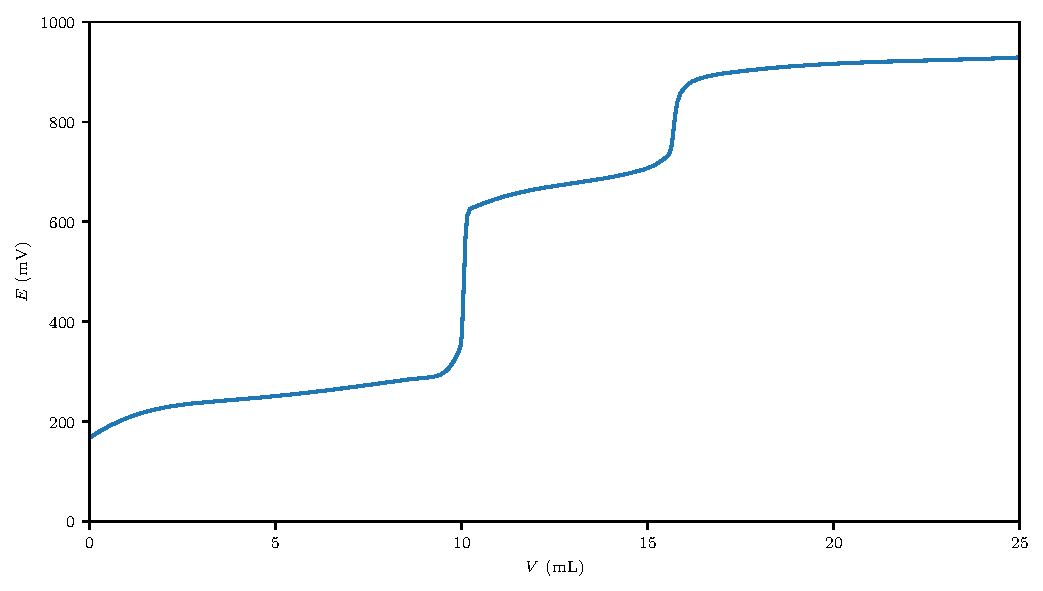
\includegraphics[width=\linewidth]{chimiePC/gene/dosage_ophen.pdf}\vspace{-1em}
    \caption{Dosage potentiométrique de la solution par le sulfate cérique.}
\end{figure}

\begin{questions}
\questioncours Quels types d'électrodes sont utilisées pour ce dosage?

\question Écrire les deux équations de dosage qui peuvent avoir lieu. Calculer leurs constantes d'équilibre. Est-ce cohérent avec la courbe de dosage observée expérimentalement?

\begin{EnvUplevel}
En réalité, les ions Fe$^{3+}$, Fe$^{2+}$, Co$^{3+}$ et Co$^{2+}$ forment avec l'orthophénanthroline des complexes très stables de formule générale [M(o-phen)$_3$]$^{n+}$.
Les ions Ce$^{4+}$ et Ce$^{3+}$ ne forment pas de complexe avec l'orthophénanthroline.  

\end{EnvUplevel}
\question Calculer la quantité de matière d'orthophénanthroline. 

\question En déduire les espèces (potentiellement) en solution avant le dosage et en déduire les réactions de dosage qui ont réellement lieu. 
\question Déterminer l'ordre des réactions de dosage.

\question En déduire la concentration en ions cobalt ainsi que les potentiels standard des deux couples impliqués dans le dosage. On supposera que tout le colbalt est complexé.

\question Que peut-on en déduire sur les constantes globales de formation des complexes considérés?
\end{questions}

\paragraph{Données : } potentiels standards $E^\circ$ dans les CNTP (en l'absence de tout agent complexant)
\begin{center}\begin{tabular}{rccc}
    \hline
    & $\mathrm{{Fe^{3+}}_{(aq)} \,/\, {Fe^{2+}}_{(aq)}}$ & $\mathrm{{Co^{2+}}_{(aq)} \,/\, {Co^{2+}}_{(aq)}}$ & $\mathrm{{Ce^{4+}}_{(aq)} \,/\, {Ce^{3+}}_{(aq)}}$ \\
    $E^\circ$ (V) & 0,77 & 1,84 & 1,44 \\ \hline\hline 
\end{tabular}\end{center}

\'Electrode au calomel saturé (ECS) : $E_\text{ref} = 244$ mV ;

On note: $e^\circ = \dfrac{RT}{\scr{F}} \ln10 = 59$ mV ; \\[-.2em]

o-phen : {\setchemfig{atom sep = 1.5 em}\chemfig{[:-30]*6(-=N-*6(-*6(-N=-=-)=-=-)=-=)}}.

\end{exercise}


\begin{solution}
\begin{questions}
\questioncours cf. cours. L'électrode de platine est une électrode du 3ème type et l'électrode de référence (au calomel saturé) est une électrode du 2ème type.

\question 
Les réactions de dosage qui peuvent avoir lieu sont :
\begin{align}
    \mathrm{Fe^{2+} + Ce^{4+}} &\longrightarrow \mathrm{Fe^{3+} + Ce^{3+}}, \tag{1} \\
    \mathrm{Co^{2+} + Ce^{4+}} &\longrightarrow \mathrm{Co^{3+} + Ce^{3+}}. \tag{2}
\end{align}

D'après la formule du cours,
\begin{align*}
    \log(K_1) &= \dfrac{E^\circ\qty\big(\mathrm{Ce^{4+} / Ce^{3+}}) - E^\circ\qty\big(\mathrm{Fe^{3+} / Fe^{2+}})}{e^\circ} = 11.2, \\
    \log(K_2) &= \dfrac{E^\circ\qty\big(\mathrm{Ce^{4+} / Ce^{3+}}) - E^\circ\qty\big(\mathrm{Co^{3+} / Co^{2+}})}{e^\circ} = -6.67.
\end{align*}
On a donc $K_1 \gg 1 \gg K_2$. La seule réaction qu'on devrait observer est donc la réaction (1). 

Or d'après la courbe de dosage, on observe deux équivalences donc deux réactions de dosage. Il se passe donc autre chose.

\question $n(\text{o-phen}) = \dfrac{1,8}{180} = 10$ mmol, alors que  $n(\mathrm{Fe^{2+}}) = 0,6$ mmol. La réaction de complexation du fer s'écrit :
$$\mathrm{Fe^{2+} + 3 \text{o-phen} \longrightarrow Fe(\text{o-phen})_3^{2+}.}$$

L'orthophénanthroline est donc en large excès par rapport au fer(II) et la réaction de complexation est quantitative. 
Il n'y a donc plus de Fe$^{2+}$ libres en solution, ils sont tous complexés.  

\question Avant le dosage sont présents en solution : le complexe Fe(o-phen)$_3^{2+}$, le complexe Co(o-phen)$_3^{2+}$ et éventuellement de l'orthophénanthroline libre (si tout le cobalt est complexé et qu'il y a un excès de ligand) ou alors du cobalt(II) libre (si tout le cobalt n'est pas complexé). 

Dans tous les cas, l'orthophénanthroline ne réagit pas avec les ions cérium(IV) et la réaction entre les ions cérium(IV) et les ions cobalt(II) libres n'a pas lieu. 

Les deux réactions de dosage correspondants aux deux équivalences observées sont donc :
\begin{align}
    \mathrm{Fe(\text{o-phen})_3^{2+} + Ce^{4+}} &\longrightarrow \mathrm{Fe(\text{o-phen})_3^{3+} + Ce^{3+}}, \tag{3} \\
    \mathrm{Co(\text{o-phen})_3^{2+} + Ce^{4+}} &\longrightarrow \mathrm{Co(\text{o-phen})_3^{3+} + Ce^{3+}}. \tag{4}
\end{align}

\question On connait la concentration en ions Fe$^{2+}$ et donc en Fe(o-phen)$_3^{2+}$ et on peut donc calculer le volume équivalent correspondant :
$$[\mathrm{Fe(\text{o-phen})_3^{2+}}] \times V_\text{tot} = [\mathrm{Ce^{4+}}] \times V_\text{eq} \quad \Longleftrightarrow \quad V_\text{eq} = 6 \text{ mL}.$$

Graphiquement on obsverse que $V_\text{eq1} = 10$ mL et $V_\text{eq2} - V_\text{eq1} = 6$ mL. 

C'est donc le dosage du cobalt complexé qui correspond à la première équivalence et la deuxième équivalence correspond au fer complexé.

\question Si on considère que tous les ions cobalt sont complexés, on a à la première équivalence :
$$[\mathrm{Co(\text{o-phen})_3^{2+}}] \times V_\text{tot} = [\mathrm{Ce^{4+}}] \times V_\text{eq1} \quad \Longleftrightarrow \quad [\mathrm{Co^{2+}}] = 5 \times 10^{-2} \mathrm{ mol\cdot L^{-1}},$$
ce qui est bien cohérent avec l'hypothèse que tous les cobalt sont complexés. 

On peut également déterminer graphiquement les $E^\circ$ des couples Fe(o-phen)$_3^{3+}$/Fe(o-phen)$_3^{2+}$ et Co(o-phen)$_3^{3+}$/Co(o-phen)$_3^{2+}$. En effet, à la demi-équivalence on a $\Delta E_{1/2\text{eq}}=E^\circ - E_\text{ref}$.

$$\text{Pour } V = \dfrac{\text{V}_\text{eq1}}{2} = 5 \text{ mL, on a } \Delta E  = E^\circ\qty\big(\text{Co(o-phen)}_3^{3+}/\text{Co(o-phen)}_3^{2+}) - E_\text{ref} \simeq 0,12 \text{ V},$$

d'où  $E^\circ(\text{Co(o-phen)}_3^{3+}/\text{Co(o-phen)}_3^{2+}$=0,36 V. 
$$\text{De même pour } V = \dfrac{\text{V}_\text{eq1}}{2} = 5 \text{ mL, on a } \Delta E  = E^\circ\qty\big(\text{Fe(o-phen)}_3^{3+}/\text{Fe(o-phen)}_3^{2+}) - E_\text{ref} \simeq 0,80 \text{ V},$$

d'où  $E^\circ(\text{Fe(o-phen)}_3^{3+}/\text{Fe(o-phen)}_3^{2+}$=1,04 V.

\question Soit M un métal (Fe ou Co), on note $\beta_{II}$ la constante de formation du complexe [M(o-phen)$_3$]$^{2+}$ et $\beta_{III}$ celle du complexe [M(o-phen)$_3$]$^{3+}$.

On montre que E$^\circ$(M(o-phen)$_3^{3+}$/M(o-phen)$_3^{2+}$) = E$^\circ$(M$^{3+}$/M$^{2+}$) + 0,06log($\frac{\beta_{II}}{\beta_{III}})$. 

Dans le cas du cobalt, E$^\circ$(Co(o-phen)$_3^{3+}$/Co(o-phen)$_3^{2+}$) < E$^\circ$(Co$^{3+}$/Co$^{2+}$). On a donc $\beta_{III} > \beta_{II}$. 

A l'inverse, pour le fer, E$^\circ$(Fe(o-phen)$_3^{3+}$/Fe(o-phen)$_3^{2+}$) > E$^\circ$(Fe$^{3+}$/Fe$^{2+}$). On a donc $\beta_{III} < \beta_{II}$.


\end{questions}
\end{solution}